% @HEADER
% ***********************************************************************
% 
%            Trilinos: An Object-Oriented Solver Framework
%                 Copyright (2001) Sandia Corporation
% 
% Under terms of Contract DE-AC04-94AL85000, there is a non-exclusive
% license for use of this work by or on behalf of the U.S. Government.
% 
% This library is free software; you can redistribute it and/or modify
% it under the terms of the GNU Lesser General Public License as
% published by the Free Software Foundation; either version 2.1 of the
% License, or (at your option) any later version.
%  
% This library is distributed in the hope that it will be useful, but
% WITHOUT ANY WARRANTY; without even the implied warranty of
% MERCHANTABILITY or FITNESS FOR A PARTICULAR PURPOSE.  See the GNU
% Lesser General Public License for more details.
%  
% You should have received a copy of the GNU Lesser General Public
% License along with this library; if not, write to the Free Software
% Foundation, Inc., 59 Temple Place, Suite 330, Boston, MA 02111-1307
% USA
% Questions? Contact Michael A. Heroux (maherou@sandia.gov) 
% 
% ***********************************************************************
% @HEADER

\documentclass[10pt,relax]{SANDreport}
\usepackage{amsmath,amsthm}
\usepackage{amssymb}
\usepackage{amsfonts}
\usepackage{palatino}

\def\choicebox#1#2{\noindent$\hphantom{th}$\parbox[t]{1.8in}{\sf
#1}\parbox[t]{4.5in}{#2}\\[0.8em]}

\author{Marzio Sala, Micheal Heroux\\
Computational Mathematics and Algorithms Department \\
Sandia National Laboratories \\
P.O. Box 5800 \\
Albuquerque, NM 87185-1110 \\[10pt]
William F. Spotz \\[10pt]
Eric T. Phipps \\[10pt]
}

\title{An Overview of PyTrilinos (DRAFT)}
\SANDnum{SAND2005-XXXX}
\SANDauthor{
Marzio Sala, William F. Spotz, Eric T. Phipps, Micheal A. Heroux}

\SANDprintDate{June 2005}
\SANDreleaseType{Unlimited Release}

\newcommand{\PyTrilinos}{{PyTrilinos}}
\newcommand{\Trilinos}{{Trilinos}}
\newcommand{\TrilinosTM}{Trilinos \copyright}
\newcommand{\trilinos}{{Trilinos}}
\newcommand{\ifpack}{{Ifpack}}
\newcommand{\aztecoo}{{AztecOO}}
\newcommand{\amesos}{{Amesos}}
\newcommand{\epetra}{{Epetra}}
\newcommand{\ml}{{ML}}
\newcommand{\mb}[1]{{\mathbf {#1} }}
\newcommand{\teuchos}{{Teuchos}}
\newcommand{\triutils}{{Triutils}}
\newcommand{\metis}{{METIS}}

\newcommand{\ie}{i.e., }
\newtheorem{assumption}{Assumption}[section]
\newtheorem{lemma}{Lemma}[section]
\newtheorem{proposition}{Proposition}[section]
\newtheorem{corollary}{Corollary}[section]
\newtheorem{theorem}{Theorem}[section]
\newtheorem{algorithm}{Algorithm}[section]
\newtheorem{definition}{Definition}[section]
\newtheorem{property}{Property}[section]
\newtheorem{interface}{Interface}[section]
\newtheorem{remark}{Remark}

\def\choicebox#1#2{\noindent$\hphantom{th}$\parbox[t]{3.0in}{\sf
#1}\parbox[t]{3.35in}{#2}\\[0.8em]}

\begin{document}

\maketitle

\begin{abstract}
PyTrilinos is a collection of Python modules that are useful for serial and
parallel scientific
computing. This collection contains modules that cover basic
dense serial linear algebra (vectors, matrices), 
distributed sparse linear algebra (vectors, multi-vectors, graphs, matrices), 
direct and iterative solution techniques for linear systems, and several
domain decomposition and multilevel
preconditioners. Also included are input/output routines to read and write
distributed linear algebra objects,
gathering a variety of
high-level distributed sparse linear algebra functionalities together.
For some objects, PyTrilinos also implements the popular Numeric module.

To run in parallel, PyTrilinos simply requires a standard Python interpreter.
The fundamental MPI calls are wrapped and included in the Epetra module, then
all intra-processor communication are handled using Epetra communicators. This
makes serial and parallel scripts using PyTrilinos virtually identical.

By using a set of properly defined interfaces, we show that it is possible to
take advantage of already available non-Python libraries. This hybrid framework
uses Python as front-end, and efficient C++ libraries for all computationally
expensive tasks. Thus, we take advantage of both the flexibility and easiness
of usage of Python, and the efficiency of the underlying C++, C and FORTRAN
code underneath. 
\end{abstract}

\clearpage
\section*{Acknowledgments}
The authors would like to acknowledge the support of the ASCI and LDRD
programs that funded development of Trilinos, and all the Trilinos developers
for their contribution to Trilinos, without which PyTrilinos will not exist.

\medskip

\SANDmain
\tableofcontents
\newpage

%-----------------------------------------------------------------------------
\section{Introduction}
\label{chap:introduction}
%-----------------------------------------------------------------------------

In high-performance scientific computing, software is usually developed using
languages like FORTRAN 77, FORTRAN 90, C or C++. If properly used, such
languages result in fast code, that allows very high flop rate. The price to
be paid is a somehow complex program, that can be difficult to develop, test,
maintain, and extend. To solve this problem, one has to note that, for most
applications, the time-critical portion of the code that requires the
efficiency of a compiled language is condifed to a small set of
self-contained functions or classes. Therefore, one can adopt an interpreted
(and possibly interactive) language, without a big performance degradation.

We felt Python to be the language of choice for this task. Python is an
interpreted, interactive, object-oriented programming language, which combines
remarkable power with very clear syntax. Since Python is an interpreted
language, it is not well suited for high-performance computing, out of the
box. However, Python can be easily extended using modules writted in C or C++
for all performance critical tasks.
\smallskip

Python has emerged as an excellent choice for scientific computing because of
its simple syntax, ease of use, and elegant multi-dimensional array
arithmetic. Its interpreted evaluation allows it to serve as both the
development language and the command line environment in which to explore
data. Python also excels as a "glue" -- a common need in the scientific arena.

PyTrilinos is a collection of mathematical algorithms and utility functions
built on top of the Trilinos project~\cite{Trilinos-home-page}.  It adds
significant power to the interactive Python session by exposing the user to
high-level commands and classes for the creation, handling and usage of serial
dense and distributed sparse linear algebra objects. Using PyTrilinos, an
interactive Python session becomes a powerful data-processing and
system-prototyping environment that can be used to test, validate, use and
extend serial and parallel numerical algorithms.

\smallskip

This document provides an overview of PyTrilinos, version 2.x.  The 2.x
versions are completely revised and not compatible with earlier releases. The
major difference is a much wider coverage of Trilinos components. Some general
Python facility is assumed such as could be acquired by working through the
tutorial in the Python distribution~\cite{python-tutorial}.  It also is
assumed that the reader is somehow familiar with Trilinos, and knows how to
install it.  It is of paramount importance to remember that PyTrilinos is
``only'' a wrapper to Trilinos, and therefore you cannot really understand
PyTrilinos if you are unfamiliar with Trilinos.  We suggest
documents~\cite{Trilinos-tutorial} to become familiar with the basic Trilinos
capabilities.

The main goal of this guide is to let you understand how to ``translate'' the
Trilinos constructs in PyTrilinos, and explain the most important differences.
The guide is {\sl not} a complete reference. If a set of options is available
for a given class of package, these options are not described here. The reader
still need to consult the manual of the underlying Trilinos package for a more
detailed insight.

%\begin{center}
%\includegraphics[height=4cm]{PyTrilinos.eps}
%\end{center}

%-----------------------------------------------------------------------------
\section{Project Overview}
\label{sec:overview}
%-----------------------------------------------------------------------------

In recent years, the application of object-oriented (OO) programming
techniques in developing software for the numerical solution of partial
differential equations (PDEs) has received increasing attention. The C++
programming language, which is widely used in developing OO PDE software, has
inherent features that are well suited for the compiled process of numerical
PDE solution.

By adopting a ``classical'' programming, in languages such as C, C++ and
FORTRAN, the programmer can  obtain high performance codes, that are at the
same quite portable (since these languages are reasonably well standarized).
However, the price to pay is a constant care to low-level system programming,
  like memory allocation and deallocation. Because compilation and linking are
  essential steps, the development cycle can be slowed down by possible bugs.
  Besides that, operations like the development of a user interface, or
  visualization of data can require a substantial amount of time. The use of
  object-oriented (OO) programming has substantially relieved the programmer
  from most of these burdens, but there is still room for improvement.

What we are interested in is a high-level programming environment, which is
flexible, but with performances comparable with that of native C, C++ or
FORTRAN code. Flexibility is fundamental to allow rapid prototyping, in the
sense that the developer should be able to write a basic code satisfying his
or her needs in a very short time. 

It is almost impossible for a single
programming language to be at the same time easy-to-use, allow fast
development, and produce optimized executables. As a matter of fact, the
goals of efficiency and flexibility clash. 

A way to satisfy these requirements is to develop a framework based on Python.
In our opinion, Python naturally complements system
languages like C, C++ and FORTRAN rather than competing with them.

Python is a high-level general purpose programming language. Because code is
automatically compiled to byte code and executed, Python is suitable for use
as a scripting language.  In tytpical Python development, a system's frontend
and infrastacture may be written in Python for ease of development and
modification, but the kernel is still written in C or C++ for efficiency.  We
use Python as a glue between different modules, written in high-performance
languages; each of these modules is an already available library, dynamically
loaded by Python when required.

PyTrilinos is a multilevel framework that take advantage of several
programming languages at different levels. 
The key components of our framework are the:
\begin{enumerate}
\item {\bf Trilinos}, a legacy code which allows high-performance scalable
linear algebra operations for problems defined on sparse matrices. Trilinos
contains more that half a million of code lines, and it can interface to
several third-party libraries. 
{\bf COUNT THE LINES???}

\item {\bf Numeric}, a well-established Python module to handle matrices and
vectors; see~\cite{numeric}.
\item {\bf SWIG}, the Simplified Wrapper and Interface Generator, which
is a  preprocessor
that turns ANSI C/C++ declarations into scripting language interfaces, and
produces a fully working Python extension module; see~\cite{swig}.
\end{enumerate}

Python combines remarkable power with very clear syntax. It has modules,
  classes, exceptions, very high-level dynamic data types, an automatic
  memory manager which frees the user from most hassles of memory management,
  and much more. Python also has some features that make it possible to write
  large programs, even though it lacks most forms of compile-time checking: a
  program can be constructed out of modules, each of which defines its own
  namespace. Exception handling makes it possible to catch errors where
  required without cluttering the code with error checking. 


%-----------------------------------------------------------------------------
\section{PyTrilinos Organization}
\label{sec:organization}
%-----------------------------------------------------------------------------

PyTrilinos reflects the Trilinos organization by presenting
a series of {\sl modules}, each of them wraps a given Trilinos package.
Algorithmic capabilities are defined within independent packages; a {\sl
  package} is an integral unit usually developed by a small team of experts in
  a particular area. 

The modules of PyTrilinos are:
\begin{enumerate}
\item {\tt Epetra.} Python wrapper for Epetra. Epetra is a collection
of concrete classes that supports the construction and use of vectors, sparse
graphs, and dense and sparse matrices. It provides serial, parallel and
distributed memory capabilities. It uses the BLAS and LAPACK where possible,
  and as a result has good performance characteristics.

Epetra is the
``language'' of Trilinos, and offers a convenient set of interfaces to define
distributed linear algebra objects. Epetra supports double-precision floating
point daata only (no single-precision or complex). 
You cannot use PyTrilinos without the Epetra module.
%
\item {\bf EpetraExt.} This module offers input/output
capabilities, making it possible to read a matrix in Harwell/Boeing or
MatrixMarket format, or to read and write generic Epetra objects 
(like maps, matrices and vectors).
%
\item {\bf Triutils.} This module allows the creation of several matrices, 
  like the MATLAB's {\tt gallery} function, and it can be useful for examples
  and testing.
%
\item {\bf Amesos.} This module contains a set of clear and consistent
interfaces with several third-party serial and parallel sparse direct solvers
(in particular,
UMFPACK~\cite{umfpack-manual},
PARDISO~\cite{pardiso-manual},
TAUCS~\cite{taucs-manual},
SuperLU and SuperLU\_DIST~\cite{superlu-manual},
DSCPACK~\cite{dscpack-manual}, and 
MUMPS~\cite{mumps-manual}). As such, PyTrilinos makes it possible to access
state-of-the-art direct solver algorithms developed by group of specialists,
  and written in different languages (C, FORTRAN77, FORTRAN90).
We refer to the Amesos reference guide~\cite{Amesos-Reference-Guide} for more details.
%
\item {\bf AztecOO.} This module contains preconditioned Krylov accelerators,
  like CG, GMRES and several others, based on the popular Aztec library.
  One-level domain decomposition preconditioners based on incomplete
  factorizations are available.
%
\item {\bf IFPACK.} This module contain object-oriented algebraic preconditioing
classes, compatible with Epetra and AztecOO.
It supports construction and use of parallel distributed memory preconditioners
such as overlapping Schwarz domain decomposition with several local solvers.
{\tt IFPACK} can take advantage of SPARSKIT~\cite{sparskit}.
%
\item {\bf ML.} This module contains a set of multilevel preconditioners based
on aggregation procedures for serial and vector problems. {\tt ML} can take
advantage of the 
METIS~\cite{metis}
ParMETIS~\cite{parmetis} libraries to create the aggregates.
For a general introduction to ML and its applications, we refer to
the ML Users Guide~\cite{ml-guide}, and to the ML web site.
\end{enumerate}

\begin{remark}
Note that all third-party libraries (except BLAS and LAPACK) are optional and
do not need to be installed to use PyTrilinos (or Trilinos).
\end{remark}

%-----------------------------------------------------------------------------
\section{Serial and Parallel Environments}
\label{sec:serial}
%-----------------------------------------------------------------------------

Research has been conducted to parallelizing Python applications: 
\begin{itemize}
\item {\bf MPI Python} is a framework for developing parallel Python
applications using MPI~\cite{MPI-Python};
\item {\bf PyPAR}  is a more light-weight wrapper of the MPI library for
Python~\cite{pypar}.
\item {\bf Python BSP} supports the more high-level Bulk Synchronous Parallel
approach~\cite{FIXME}
\end{itemize}

In all these approaches, additional overhead is introduces by the Python
interface. We decided to ...



After configuring and compiling Trilinos, one must install Trilinos 
(by typing \verb!make install!), in order to create PyTrilinos module.
The installing procedure will copy all the Python modules in a subdirectory of
the directory specified with option \verb!--prefix=<inst-dir>!, for example
\verb!lib/python2.3/site-packages/PyTrilinos!. You might want to add this
directory to your \verb!PYTHONPATH! variable, for example in bash shell
\begin{verbatim}
% export PYTHONPATH=$PYTHONPATH:\
  <inst-dir>/lib/python2.3/site-packages/PyTrilinos
\end{verbatim}

If Trilinos was configured in serial mode, to use PyTrilinos  simply type
\begin{verbatim}
% python
Python 2.3 (#1, Sep 13 2003, 00:49:11) 
[GCC 3.3 20030304 (Apple Computer, Inc. build 1495)] on darwin
Type "help", "copyright", "credits" or "license" for more information.
>>> from PyTrilinos import <module-name>
\end{verbatim}
where \verb!<module-name>! is the name of the PyTrilinos module to be
imported, as later described.

If Trilinos was configured in parallel (MPI) mode, you cannot run PyTrilinos
interactively, and you must create a script file. You can run PyTrilinos by
using an instruction of type
\begin{verbatim}
% mpirun -np 4 python ./my-script.py
\end{verbatim}
where \verb!my-script.py! contains the instruction \verb!from PyTrilinos import <module-name>!.

Within PyTrilinos, all intra-processor communication are handled though the
communicator object Epetra.Comm, a pure virtual class. A concrete object can
be defined as follows:
\begin{verbatim}
Comm = Epetra.PyComm()
\end{verbatim}
which returns an Epetra.SerialComm if PyTrilinos has been compiled in serial
mode, or an Epetra.MpiComm if PyTrilinos has support for MPI. By using
Epetra.PyComm, PyTrilinos scripts are virtually identical for both serial and
parallel runs, and generally reads:
\begin{verbatim}
Epetra.MpiInit()
Comm = Epetra.PyComm()
...
Epetra.MpiFinalize()
\end{verbatim}

%-----------------------------------------------------------------------------
\section{Using PyTrilinos}
\label{sec:using}
%-----------------------------------------------------------------------------

All Epetra distributed objects requires a suitable map, which basically
contains the set of locally hosted elements.
For parallel computations, we suppose to use $N_p$ processors. The linear
algebra objects $A$, $X$ and $B$ are distributed among the processors so that
each row is assigned to exactly one processor. The data layout is determined
by the so-called maps (see Section~\ref{sec:maps}). Here, we suppose that the
maps of $A$, $X$ and $B$ are all equivalent; this means that if row $i$ of $A$
is contained on processor $j$, then also the row $i$ of $X$ and $B$ are
contained on the same processor.

\smallskip

Once a Map has been created, distributed vectors are created and used as follows:
\begin{verbatim}
>>> X = Epetra.Vector(Map)
>>> for i in range(0, X.MyLength()):
...   X[i] = i
... 
>>> print X
[ 0.  1.  2.  3.  4.  5.  6.  7.  8.  9.]
\end{verbatim}
Multi-vectors (that is, a collection of vectors all sharing the same Map) can
be created using typical Epetra constructors. Several methods cab be used to
access and modify vectors and multivectors.  To set all the elements of a
vector to a given value simply use {\tt X.PutScalar(0.0)}. To define random
elements, use {\tt X.Random()}.

\smallskip

Epetra provides an extensive set of classes to create and fill
distributed sparse matrices. These classes allow row-by-row or
element-by-element constructions. Support is provided for common matrix
operations, including scaling, norm, matrix-vector multiplication and
matrix-multivector multiplication.
Using Epetra objects, applications do not need to know about the
particular storage format, and other implementation details such as data
layout, the number and location of ghost nodes. 

The process of creating a sparse matrix is more involved than the
process for dense matrices. This is because, in order to obtain
excellent numerical performance, one has to provide an estimation of
the nonzero elements on each row of the sparse matrix. (Recall that
dynamic allocation of new memory and copying the old storage into the
new one is an expensive operation.)

As an example, in this Section we will present how to construct a
distributed (sparse) matrix, arising from a finite-difference solution
of a one-dimensional Laplace problem. This matrix looks like:
\begin{equation*}
A = \begin{pmatrix}
 2 & -1 &     &   &    \\
-1 &  2     & -1     &        &    \\
   & \ldots & \ldots & \ldots & -1 \\
   &        &        & -1     & 2
\end{pmatrix}.
\end{equation*}
The example illustrates how to construct the matrix,
and how to perform matrix-vector operations.

Then, we have to specify the number
of nonzeros per row. In general, this can be done in two ways:
\begin{itemize}
\item Furnish an integer value, representing the number of nonzero
  element on each row (the same value for all the rows);
\item Furnish an integer vector \verb!NumNz!, of length
  \verb!NumMyElements()!, containing the nonzero elements of each row.
\end{itemize}

We present here how to proceed using the first approach:
\begin{verbatim}
>>> A = Epetra.CrsMatrix A(Epetra.Copy,Map,3);
\end{verbatim}
We can now create the matrix, by adding one row at-a-time.
To fill its values, we
need some additional variables: let us call them \verb!Indexes! and
\verb!Values!. For each row, \verb!Indices! contains global column
indices, and \verb!Values! the correspondingly values.
\begin{verbatim}
for i in range(0, n):
  if i == 0:
    Indices = [i, i + 1]
    Values  = [2.0, -1.0]
  elif i == n - 1:
    Indices = [i, i - 1]
    Values  = [2.0, -1.0]
  else:
    Indices = [  i,  i - 1, i + 1]
    Values  = [2.0,   -1.0,  -1.0]
  Matrix.InsertGlobalValues(i, Values, Indices)
ierr = Matrix.FillComplete()
\end{verbatim}
Finally, we transform the matrix representation into one based on local
indexes. The transformation in required in order to perform efficient parallel
matrix-vector products and other matrix operations.

This call to \verb!FillComplete()! will reorganize the internally stored
data so that each process knows the set of internal, border and external
elements for a matrix-vector product of the form $B = AX$. Also, the
communication pattern is established. As we have specified just one map,
Epetra considers that the the rows of $A$ are distributed among the
processes in the same way of the elements of $X$ and $B$.

Another useful class is {\tt Epetra.FECrsMatrix}.
The most important additional feature provided by the
Epetra.FECrsMatrix with respect to Epetra.CrsMatrix, is the capability
to set non-local matrix elements. 

\smallskip

Once a (square) sparse matrix and two vectors are created, an important
problem is how to solve the corresponding linear system
\begin{equation}
\label{eq:lin_sys}
A X = B
\end{equation}
where $A \in \mathbb{R}^{n \times n}$ is a sparse linear operator, $X \in
\mathbb{R}^{n \times m}$ and $B \in \mathbb{R}^{n \times m}$ are the solution
and right-hand side, respectively. $n$ is the global dimension of the problem,
  and $m$ is the number of vectors in the multi-vectors $X$ and $B$. 
  (If $m = 1$, then $X$ and $B$ are ``normal'' vectors.)
Linear systems of type (\ref{eq:lin_sys}) arise in a variety of applications,
  and constitute the innermost computational kernel, and often the most
  time-consuming of several numerical algorithsm. An efficient solver for
  Equation (\ref{eq:lin_sys}) is of fundamental importance for most PDE
  solvers, both linear and non-linear.

\smallskip

Probably, the most robust strategy to solve (\ref{eq:lin_sys}) is to factorize
the linear matrix $A$ into the product of two matrices $L$ and $U$, so that
$A = L \, U$, and 
the linear systems with $L$ and $U$ are readily solvable. Typically,
$L$ and $U$ are a lower and upper triangular matrix, respectively, and the
process is referred to as Gaussian elimination. 

All Amesos objects are constructed from the function class
\verb!Amesos!.  Amesos allows a code to delay the
decision about which concrete class to use to implement the
Amesos.BaseSolver interface. The main goal of this class is to allow
the user to select any supported (and enabled at configuration time)
direct solver, simply changing an input parameter. Let us suppose that Amesos
has been configured and compiled with support for SuperLU. To solve the linear
system (\ref{eq:lin_sys}) with SuperLU, we first need to create a Solver
object,
\begin{verbatim}
>>> Factory = Amesos.Factory()
>>> Solver = Factory.Create("Superlu", Problem)
\end{verbatim}
Then, we can perform the symbolic and numeric factorizations using methods
\begin{verbatim}
>>> Solver.SymbolicFactorization()
>>> Solver.NumericFactorization()
\end{verbatim}
The numeric factorization phase will check whether a symbolic
factorization exists or not. If not, method
\verb!SymbolicFactorization()! is invoked.  Solution is computed (after
setting of LHS and RHS in the linear problem), using
\begin{verbatim}
>>> Solver.Solve()
>>> del Solver
\end{verbatim}
The solution phase will check whether a numeric factorization exists or
not. If not, method \verb!NumericFactorization()! is called.
Users must provide the nonzero structure of the matrix for the symbolic
phase, and the actual nonzero values for the numeric
factorization. Right-hand side and solution vectors must be set before
the solution phase.
  
Several parameters are available to toggle the selected Amesos solver.
To specify parameters, one can use Python's dictionaries:
\begin{verbatim}
>>> Factory = Amesos.Factory();
>>> Solver = Factory.Create(Type, Problem);
>>> AmesosList = {
...  "PrintTiming": ("bool", "true"),
...  "PrintStatus": ("bool", "true")
... }
...
>>> Solver.SetParameters(AmesosList);
\end{verbatim}
Please consult the Amesos manual~\cite{Amesos-Reference-Guide} for more
details.

\bigskip

For sparse matrix, the major inconvenience of direct solution methods is that
the $L$ and $U$ factors are typically much denser than the original matrix
$A$, making Gaussian elimination too memory demanding for large scale
problems. Moreover, the factorization process is inherintly serial, and
parallel factorization algorithms can be successfully used only with a
relatively modest number of processors. The
forward and back triangular solves typically exhibit very poor parallel speedup.

A very well known solution to this problem is to adopt an iterative solution
process, like conjugate gradient or GMRES~\cite{FIXME}. The rationale behind
iterative methods is that they only require (at least in their simplest form)
matrix-vector and vector-vector products, and both operations scale well for
sparse matrices. 

To adopt an non-preconditioned iterative solver (for example, CG), with 1550
maximum iterations and a tolerance of $10^{-5}$ on the relative residual,
  PyTrilinos requires the following instructions:
\begin{verbatim}
>>> Solver = AztecOO.AztecOO(Matrix, LHS, RHS)
>>> Solver.SetAztecOption(AztecOO.AZ_solver, AztecOO.AZ_cg)
>>> Solver.SetAztecOption(AztecOO.AZ_precond, AztecOO.AZ_none)
>>> Solver.Iterate(1550, 1e-5)
\end{verbatim}

Unfortunately, the convergence of
iterative methods is determined by the spectral properties of the matrix $A$
(typically, its condition number $\kappa(A)$), and for
real-life problems $\kappa(A)$ is ``large'', meaning that the iterative
solution method will converge slowly. To solve this problem,
the original linear system is replaced by 
\[
A P P^{-1} X = B
\]
where $P$, called {\sl preconditioner}, is an operator whose inverse aim to
represent the inverse of $A$, though being much cheaper to compute.
$P$ is chosen so that $AP^{-1}$ is easier to solver than $A$ 
(that is, it is better conditioned). 

\smallskip

Often, algebraic preconditioners are adopted, that is, $P$ is constructed by
manipulating the entries of $A$. This gives rise to the so-called incomplete
factorization preconditioners (ILU) or algebraic multilevel methods. 

Because ILU preconditioners do not scale well on parallel computers, a common
practice is to perform {\em local} ILU factorizations.  In this situation,
each processor computes a factorization of a subset of matrix rows and
columns independently from all other processors.  This additional layer of
approximation leads to a block Jacobi type of preconditioner across
processors, where each block is solved using an ILU preconditioner.  The
difficulty with this type of preconditioner is that it tends to become less
robust and require more iterations as the number of processors used
increases.  This effect can be offset to some extent by allowing {\em
overlap}.  Overlap refers to having processors redundantly own certain
rows of the matrix for the ILU factorization.  Level-1 overlap is defined
so that a processor will include rows that are part of its original set.
In addition, if row $i$ is part of its original set and row $i$ of $A$ has
a nonzero entry in column $j$, then row $j$ will also be included in the
factorization on that processor.  Other levels of overlap are computed
recursively. 

What we have just described is an example of one-level overlapping domain
decomposition (DD) preconditioners.  The basic idea of DD methods consists in
dividing the computational domain into a set of subdomains, which may or may
not overlap. We will focus on overlapping DD methods only, because they can be
re-interpreted as algebraic manipulation of the assembled matrix, thus
allowing the construction of black-box preconditioners. Overlapping DD methods
are often referred to as overlapping Schwarz methods. DD preconditioners can
be written as
\begin{equation}
  \label{eq:prec_dd}
  P^{-1} = \sum_{i=1}^M R_i^T B_i^{-1} R_i,
\end{equation}
where $M$ represents the number of subdomains,
$R_i$ is a rectangular Boolean matrix that restricts
a global vector to the subspace defined by the interior of the $i$th
subdomain, and $B_i$ approximates the inverse of 
\begin{equation}
  \label{eq:aztecoo_tilde_a}
  A_i = R_i A R_i^T ,
\end{equation}
for example, being its ILU factorization.

In PyTrilinos two ways are available to define DD preconditioners:
\begin{enumerate}
\item Using the {\tt AztecOO}'s preconditioners. The specification starts with
\begin{verbatim}
Solver.SetAztecOption(AztecOO.AZ_precond, AztecOO.AZ_dom_decomp)
\end{verbatim}
Next if an incomplete factorization of $A_i$ will be used, then specify its parameters:
\begin{verbatim}
Solver.SetAztecOption(AztecOO.AZ_subdomain_solve, AztecOO.AZ_ilu)
Solver.SetAztecOption(AztecOO.AZ_graph_fill, 1)
\end{verbatim}

\item Using the {\tt IFPACK}'s preconditioners. This requires the {\tt IFPACK}
module.
\begin{verbatim}
Factory = IFPACK.Factory();
Prec = Factory.Create("IC", Matrix);
IFPACKList = {
  "fact: level-of-fill": ("int", "5")
}

Prec.SetParameters(IFPACKList);
Prec.Initialize();
Prec.Compute();
Problem = Epetra.LinearProblem(Matrix, LHS, RHS);
Solver = AztecOO.AztecOO(Problem);
Solver.SetPrecOperator(Prec)
Solver.SetAztecOption(AztecOO.AZ_solver, AztecOO.AZ_gmres);
\end{verbatim}
\end{enumerate}

\bigskip

Another class of preconditioners is given by multilevel preconditioners.
For certain combinations of iterative methods and linear systems, the
error at each iteration projected onto the eigenfunctions has components
that decay at a rate proportional to the corresponding eigenvalue (or
frequency).  Multilevel methods exploit this property \cite{Briggs2000}
by projecting the linear system onto a hierarchy of increasingly
coarsened ``meshes" so that each error component rapidly decays on at
least one coarse ``mesh."  The linear system on the coarsest ``mesh",
called the coarse grid problem, is solved exactly.  The iterative method
is called the smoother, as a reflection of its diminished role as a way
to damp out the high frequency error.  The grid transfer (or
interpolation) operators are called restriction ($\mathbf{R}$) and
prolongation ($\mathbf{P}$) operators.

Multilevel methods are characterized by the sequence of coarse spaces, the
definition of the operator each coarse space, the specification of the
smoother, and the restriction and prolongation operators.  Geometric multigrid
(GMG) methods  are multilevel methods that require the user to specify the
underlying grid, and in most cases a hierarchy of (not necessarily nested)
  coarsens grids.  Both the automatic generation of a grid-hierarchy for GMG
  and the specification of the ML, designed for unstructured problems, are
  beyond the scope of the tutorial.

Algebraic multigrid (AMG)  (see \cite[Section 8]{Briggs2000}) method
development has been motivated by the demand for multilevel methods that are
easier to use.  In AMG, both the matrix hierarchy and the prolongation
operators are constructed just from the stiffness matrix.  Recall that to use
Aztec00 or IFPACK,  a user must supply a linear system, a select a
preconditioning strategy.  In AMG, the only additional information required
from the user is to specify a coarsening strategy.

This Section requires to import the {\tt ML}, {\tt AztecOO} and {\tt Epetra}
modules. First, we set up the parameters for ML using a python dictionary:
\begin{verbatim}
>>> MLList = {
...  "max levels"        : ("int", "3"),
...  "output"            : ("int", "10"),
...  "smoother: type"    : ("string", "symmetric Gauss-Seidel"),
...  "aggregation: type" : ("string", "Uncoupled")
... };
... 
\end{verbatim}
Then, we create the preconditioner and compute it,
\begin{verbatim}
Prec = ML.MultiLevelPreconditioner(Matrix, False);
Prec.SetParameterList(MLList);
Prec.ComputePreconditioner();
\end{verbatim}
Finally, we set up the solver, and specifies to use \verb!Prec! as
preconditioner:
\begin{verbatim}
Solver = AztecOO.AztecOO(Matrix, LHS, RHS)
Solver.SetPrecOperator(Prec)
Solver.SetAztecOption(AztecOO.AZ_solver, AztecOO.AZ_cg);
Solver.SetAztecOption(AztecOO.AZ_output, 16);
Solver.Iterate(1550, 1e-5)
\end{verbatim}

\bigskip

Several utilities are available in several modules to facilitate the writing
of new scripts.
Matrices can be easily generated using module {\tt Triutils}. For
details, we refer to the Trilinos tutorial. Here, we just show how to generate
a matrix corresponding to a 3D Laplacian on a structured Cartesian grid.
Class {\tt Epetra.Time} can be used to track the elapsed CPU time.
The EpetraExt module offers matrix-matrix operations. Two matrices
(with compatible maps) can be added of multiplied. Also, reading and writing
capabilities of important Epetra objects are made available. For example, to
read a vector and a matrix stored in Matrix-Market format, one simply has to
write:
\begin{verbatim}
(ierr, X2) = EpetraExt.MatrixMarketFileToMultiVector("x.mm", Map)
(ierr, A2) = EpetraExt.MatrixMarketFileToCrsMatrix("A.mm", Map)
\end{verbatim}
These functions are a powerful tool to exchange data from a code based on
Trilinos and PyTrilinos.

Finally, some
capabilities are given to handle dense and serial linear algebra problems.
These capabilities are based on the Epetra wrapper for BLAS and LAPACK, and
therefore the serial dense module of PyTrilinos is computationally efficient.

%-----------------------------------------------------------------------------
\section{Comparison with Related Projects}
\label{sec:related}
%-----------------------------------------------------------------------------

Similar projects are:
\begin{itemize}
\item {\bf MATLAB.} Any software framework which claims to be easy-to-use
cannot avoid a comparison with MATLAB, the {\sl de-facto} standard in
numerical analysis. Our impression is that, while MATLAB's vector syntax and
built-in matrix data types greatly simplifies the programming language, it is
not possible to perform large-scale computing using this language. MATLAB's
sparse matrix operations are slow compared with Epetra's. Another handicap of
MATLAB is its inflexible language: There may be only one visible function in a
file, and the function name must be the file name itself. This can make harder
to modularize the code. Desiderable language features, such as exception
handling, are also missing in MATLAB.


\item {\bf Numeric.} Numerical Python adds a fast, compact, multidimensional array language facility to Python.
\item  {\bf NumArray.} 
Numarray is a reimplementation of Numeric which adds the ability to
efficiently manipulate large numeric arrays in ways similar to Matlab and IDL.
\item {\bf SciPy.} SciPy is an open source library of scientific tools for
Python. SciPy supplements the popular Numeric module, gathering a variety of
high level science and engineering modules together as a single package. SciPy
includes modules for graphics and plotting, optimization, integration, special
functions, signal and image processing, genetic algorithms, ODE solvers, and
others.
\item {\bf ScientificPython.} 
ScientificPython is a collection of Python modules that are useful for
scientific computing. In this collection you will find modules that cover
basic geometry (vectors, tensors, transformations, vector and tensor fields),
  quaternions, automatic derivatives, (linear) interpolation, polynomials,
  elementary statistics, nonlinear least-squares fits, unit calculations,
  Fortran-compatible text formatting, 3D visualization via VRML, and two Tk
  widgets for simple line plots and 3D wireframe models. There are also
  interfaces to the netCDF library (portable structured binary files), to MPI
  (Message Passing Interface, message-based parallel programming), and to
  BSPlib (Bulk Synchronous Parallel programming).

  This is a big project!!!!
\end{itemize}
We believe that PyTrilinos is a very unique effort, since for the first time a
massive number of high-performance algorithms for distributed sparse linear
algebra is made easily available with the scripting language Python.  None of
the previously reported projects for scientific computing with Python handles
sparse and distributed matrices. 

\smallskip

PyTrilinos is compatible with the popular Numeric module
Vectors defined as Epetra\_Vector are automatically defined as Numeric
vectors, and they can therefore be used with any Numeric function or class.
However, note that a Numeric vector is {\sl not} automatically recognized as
Epetra\_Vector, since all distributed Epetra objects requires an underlying
Map (not supported by Numeric).

\bigskip
\fbox{Say something about visualization, for example GNUPLOT}
\bigskip

Other researchers have successfully used Python for their work, although in
areas slightly different from that of PyTrilinos. 

%-----------------------------------------------------------------------------
\section{Concluding Remarks}
\label{sec:concluding}
%-----------------------------------------------------------------------------

The PyTrilinos project is an effort to facilitate the design, development,
integration and ongoing support of mathematical software libraries. 
PyTrilinos provides a simple but powerful rapid development language, along with
the integration tools needed to apply it in realistic development
environments. With PyTrilinos, it is no longer necessary to choose between fast
development and fast execution.

In our opinion, the {\bf impact} of PyTrilinos is the following:
\begin{itemize}
\item {\bf Rapid Prototyping.}
Because Python is a simple language, coding is much faster than in other
  languages. For example, its dynamic typing, built-in objects, and garbage
  collection eliminate much of the manual bookkeeping code typically required
  in languages like C or C++. Since things like type declaration, memory
  management, and common data structure implementations are absent, Pytho
  programs are typically a fraction of the sier of their C or C++ equivalents.
  Becase most bookkeeping code is missing, Python programs are easier to
  understand and more closely reflect the actual problem they're intended to
  address. 

  Python's
  develoment cycle is dramatically shorter than that of traditional tools. In
  Python, there are no compile or link steps--Python programs simply import
  modules are runtime and use the objects they contain. Because of this,
Python programs run immediately after changes are made. Python integration
  tools make it usable in hybrid, multicompont applications. As one
  consequence, systems can simultaneousl utilize the strengths of Python for
  rapid development, and of traditional languages such as C for rapid
  execution.
  This flexibility of development modes is crucial in realistic environments.
  Python is optimized for speed of development, but that alone is not enough.
%
\item {\bf Brevity.} Python codes can be short and concise. This is also
promoted by the object-oriented design of both PyTrilinos and Trilinos itself.
%
\item {\bf Modularity.} Python allows the code to be organized in reusable,
  self-contained modules.
%
\item {\bf Reusability.} Because Python is a high-level, object-oriented
language, it encourages writing reusable software and well-designed systems.
%
\item {\bf Legacy code migration.} Moving existing code from C/C++ to Python
makes it simpler and more flexible.
Modern numerical
algorithms are complex, and both the testing and fine tuning of already
developed algorithsm, or the development of brand new ones require a massive
investment, for which rapid prototyping is essential. On the other hand,
programmers simply cannot ignore efficiency completely. Our approach is the
following: use Python when speed of development matters, compiled languages
when efficiency dominates, and combinations of the two when our goals are
not absolute.
%
\item {\bf Explorative Computation.} Since Python is an interpreted and
interactive scripting language, the user can undertake computations in an
explorative manner. Intermediate results can be examined and taked into
account before the next computational step, without the compile-link-run cycle
typical of C or C++.
%
\item {\bf Integration.} Python's role as integration tool. PyTrilinos relies
on the ability to mix components written in other languages. C, C++ and
FORTRAN code is called, but note that Python coders don't need to care.
  Python lends itself to experimental, interactive program development, and
  encourages developing systems incrementally by testing components in
  isolation and putting them together later.
  By themselves, neigher C nor Python is adequate to address the development
  bottleneck; together, they can do much more. We model we are using splits
  the workplace into {\sl frontend} componenta that can benefit from Python's
  easy-of-use and {\sl backend} modules that require the efficiency of static
  languages like C, C++, or FORTRAN.
%
\end{itemize}

\smallskip

To summarize our prospective, the most important feature of Python is to be a
powerful but simple programming language designed for development speed, for
situations in which the complexity of larger languages can be a liability. Of
course, Python entusiasts will point out several other strengths of the
language; our aim was to show that Python can be successfully used also to
develop and use state-of-the-art numerical linear algebra algorithms, in both
serial and parallel environments.  Of course, Python is not the perfect for
all problems. The most important problems we have encountered are:
\begin{itemize}
\item {\bf Portability.} PyTrilinos is an open source library of scientific
  tools for Python.  It is developed concurrently on both Linux and MAC OS X,
  and it should port successfully to most other platforms where Trilinos,
  Python, Numeric and SWIG are available.
%
\item {\bf Performance Considerations.}
By using a Python wrapper a performance penalty is introduced, due to
deconding of Python script, the execution of wrapped code, and returning the
results in a Python-compliant format. These tasks may require thousands of CPU
cycles, therefore it is important to distinguish.
item The performance penalty is small if the C/C++ function does a lot of work.
Therefore, for rarely called function, this penalty is negligible.
All performance critical kernels should be written in C/C++, and
everything else can be in Python.
%
\item {\bf Main differences between Trilinos and PyTrilinos.}
Although \PyTrilinos\ mimic very closely Trilinos, there is no one-to-one
map. The most important differences are:
\begin{itemize}
\item No memory allocation and deallocation occurs in PyTrilinos.
\item No header files are required by PyTrilinos.
\item No {\tt int} and {\tt double} arrays are used by PyTrilinos, replaced instead by
Python's lists.
\item Instruction \verb!cout << EpetraObject! is replaced by \verb!print EpetraObject!.
\item \teuchos's parameters lists are replaced by Python's dictionaries.
\end{itemize}
%
\item {\bf Limited Templated Code.} Most numerical
libraries are currently adopting massive template support, and templates have
no meaning in Python. This means that the interface writer has to select {\sl
  a-priori} which instances of the templated class will be included.
%
\item {\bf Shared Libraries on Massively Parallel Computers.} Another problem
is related to the shared library approach, which is the easiest way of
intergrating third-party libraries in Python. Most massively parallel
computers do not support shared libraries, therefore making the use of Python
scripts still off-limits for very large scale computations.
%
\item {\bf Lack of Compile-time Checks.} In Python all checks must be
performed at run-time.
\end{itemize}

Finally, we point out that PyTrilinos is not meant to replace Trilinos. You
can think of PyTrilinos as a collection of all successful and stable
numerical algorithms of Trilinos.  Hence, not all the algorithms and the tools
of Trilinos are (or will) be ported to PyTrilinos. 

%-----------------------------------------------------------------------------%
\bibliographystyle{plain}
\bibliography{../UsersGuide/guide}
%-----------------------------------------------------------------------------%

\end{document}
